% This example is meant to be compiled with lualatex or xelatex
% The theme itself also supports pdflatex
\PassOptionsToPackage{unicode}{hyperref}
\documentclass[aspectratio=1610, 9pt]{beamer}

% Load packages you need here
\usepackage{polyglossia}
\setmainlanguage{german}

\usepackage{csquotes}
    

\usepackage{amsmath}
\usepackage{amssymb}
\usepackage{mathtools}

\usepackage{hyperref}
\usepackage{bookmark}

% load the theme after all packages

\usetheme[
  showtotalframes, % show total number of frames in the footline
]{tudo}

% Put settings here, like
\unimathsetup{
  math-style=ISO,
  bold-style=ISO,
  nabla=upright,
  partial=upright,
  mathrm=sym,
}

\title{\LaTeX-Beamer-Theme der TU~Dortmund}
\author[M.~Nöthe]{Maximilian Nöthe}
\institute[Kurzform Lehrstuhl]{Names des Lehrstuhls \\  Name der Fakultät}
\titlegraphic{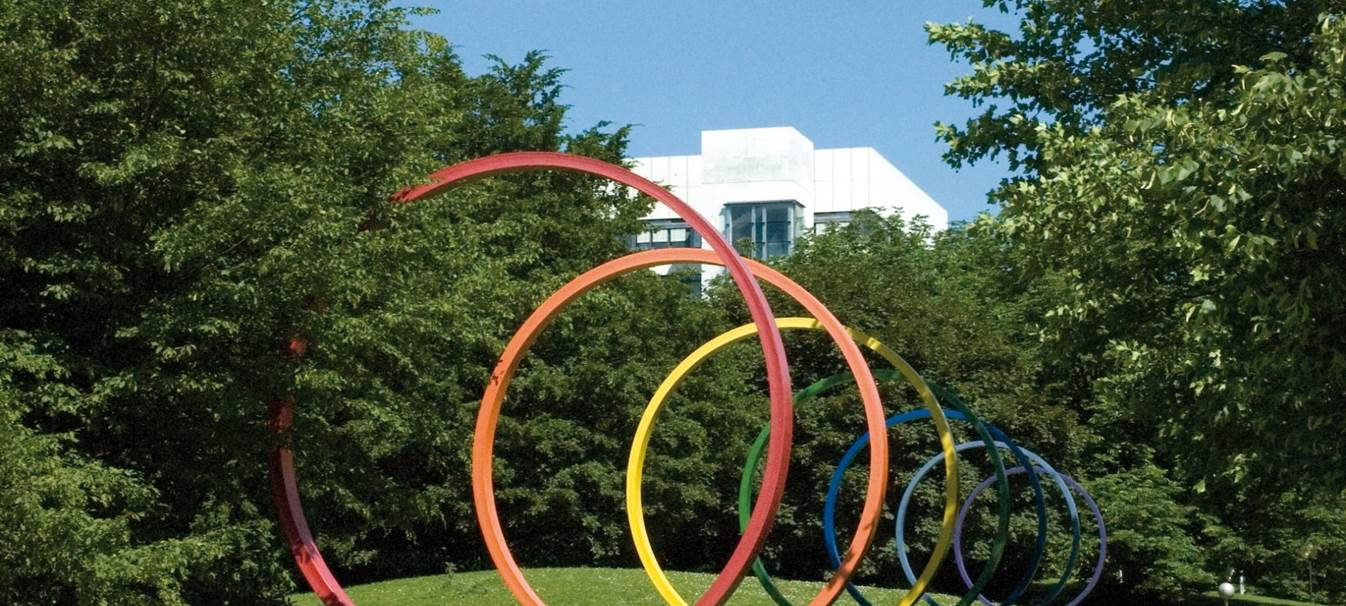
\includegraphics[width=0.7\textwidth]{images/tudo-title-2.jpg}}


\begin{document}

\maketitle

\begin{frame}{Hinweise}
  Zu diesem Theme
  \begin{itemize}
    \item Zur Installation des Themese muss mindestens die Datei \texttt{beamerthemetudo.sty} und der Ordner \texttt{logos} in einen Ordner verschoben werden, in dem \LaTeX nach Paketen sucht.
      Dies können sein
      \begin{itemize}
        \item \texttt{TEXMFHOME/tex/latex/tudobeamertheme}. Den Wert von \texttt{TEXMFHOME} bekommen sie über \texttt{kpsewhich --var-value TEXMFHOME}, üblicherweise ist dies \texttt{\$HOME/texmf}.
        \item Der gleiche Ordner in dem Sie ihr Dokument kompilieren
        \item Ein beliebiger Ordner, der in der Variablen \texttt{TEXINPUTS} enthalten ist.
      \end{itemize}
  \end{itemize}
  
  Oneliner zur Installation:\\
  \texttt{\footnotesize\$ cd `kpsewhich --var-value TEXMFHOME` \&\& git clone https://github.com/maxnoe/tudobeamertheme}

  \medskip
  Allgemein zu Beamer und Latex:
  \begin{itemize}
    \item Umfangreicher \LaTeX-Kurs von PeP et Al. \\
      \url{http://toolbox.pep-dortmund.org/notes}
    \item Latex-Beamer Dokumetation:\\
    \url{http://www.ctan.org/pkg/beamer}
  \end{itemize}
\end{frame}

\begin{frame}{Einführung}
  \tableofcontents
\end{frame}

\section{Fonts}
\begin{frame}
  Der Font der im Corporate Design der TU Dortmund vorgesehen ist,
  ist \enquote{Akkurat Office}.

  Falls dieser nicht verfügbar ist, wird als Alternative \enquote{Fira Sans}
  verwendet.

  Für Mathematik wird bei Verwendung von \texttt{xelatex} oder \texttt{lualatex} der Font \enquote{Fira Math} verwendet.
\end{frame}

\begin{frame}{Mathe}
  \begin{align*}
    \nabla \cdot \symbf{B} &= 0 &
    \nabla \cdot \symbf{E} &= \frac{ρ}{ε_0} \\
    \nabla \times \symbf{E} &= -\partial_t \symbf{B} &
    \nabla \times \symbf{B} &= μ_0 \symbf{j} + μ_0 ε_0 \partial_t \symbf{E} &
  \end{align*}
\end{frame}
\end{document}
